\documentclass{article}

\usepackage{polski}
\usepackage{amsmath, array}
\usepackage{graphicx}
\usepackage{float}
\usepackage{subfig}
\usepackage{multirow}
\usepackage{enumitem}
\usepackage{hyperref}
\usepackage{listings}

\NewDocumentCommand{\codeword}{v}{%
\texttt{#1}%
}

\title{Zadanie 1 - Optymalizacja Mnożenia Macierzy}
\author{\textbf{Łukasz Wala}\\
    \textit{AGH, Wydział Informatyki, Elektroniki i Telekomunikacji} \\
    \textit{Optymalizacja Kodu na Różne Architektury 2022/23}}
\date{Kraków, \today}


\begin{document}
\maketitle

\section{Wstęp}
Celem zadanie jest zoptymalizowania procesu mnożenia macierzy zgodnie z intrukcjami
dostępnymi pod adresem \url{github.com/flame/how-to-optimize-gemm}. Pod nim znajduje się
również kod źródłowy kolejnych kroków optymalizacji, więc w celu zachowania zwięzłości sprawozdania,
w kolejnyc etapach załączane będą jedynie adresy do odpowiednich plików. 

Testy przeprowadzano na komputerze z procesorem AMD Ryzen 7 4700u (8 rdzeni taktowanych zegarem
o podstawowej częstotliwości 2 GHz, w podstawowej konfiguracji, bez \textit{overclockingu}). Testy
wykonywano jednowątkowo. Procesor wspiera instrukcje wektorowe z rodziny SSE oraz częściowo
AVX (AVX, AVX2, natomiast już nie AVX-512). Użyty system operacyjny to Linux.

\section{Optymalizaje}
\subsection{Bazowy przypadek}

\href{https://github.com/flame/how-to-optimize-gemm/blob/master/src/HowToOptimizeGemm/MMult0.c}{Kod źródłowy}

\noindent Bazowy przypadek to mnożenie macierzy w trzech zagnieżdzonych pętlach. Do niego będą porównywane
kolejne optymalizacje. Poniższy wykres przedstawia zależność GFLOPS (liczba miliardów operacji
zmiennoprzecinkowych na sekundę) do rozmiaru macierzy.

\begin{figure}[H]
    \centering
    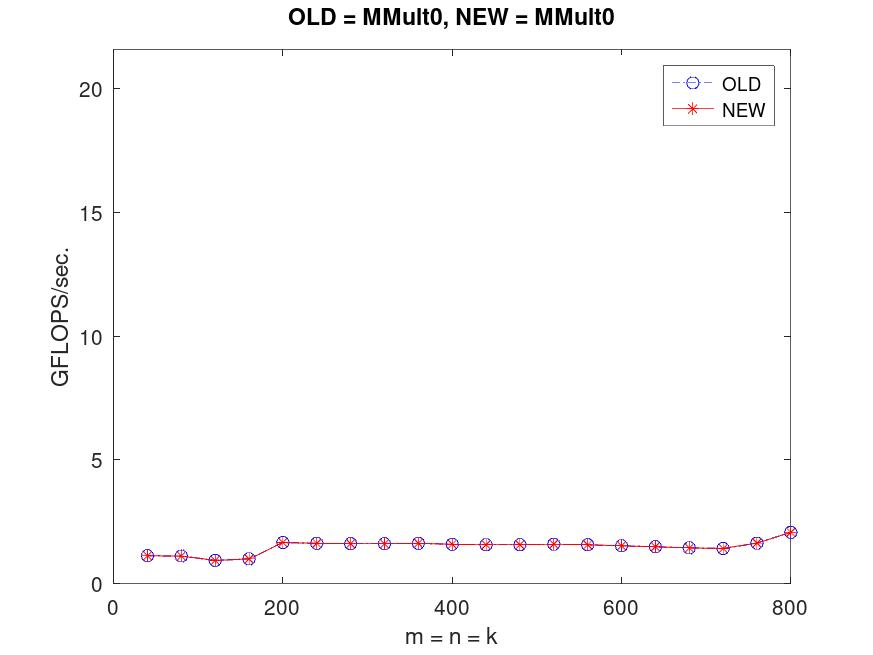
\includegraphics[width=1.0\textwidth]{figure1.jpg}
    \caption{Przypadek bazowy}
\end{figure}

\subsection{Optymalizacje 1 - 1x4\_5}

\href{https://github.com/flame/how-to-optimize-gemm/blob/master/src/MMult_1x4_5.c}{Kod źródłowy}

\noindent Pierwsze optymalizacje polegają na wydzieleniu rutyny odpowiedzialnej za mnożenie,
oraz rozwinięcie pętli. 

Można już zauważyć pewną poprawę związaną z wydzieleniem 4 iteracji
pętli do jednej, przez co wartość \codeword{p} jest aktualizowana co osiem operacji zmiennoprzecinkowych
(w przeciwieństwie do co dwie przed zmianami) oraz element \codeword{A(0,p)} jest wyciągany z pamięci
rzadziej (ma znaczenie w przypadku macierzy nie mieszczących się w \textit{cache}).

\begin{figure}[H]
    \centering
    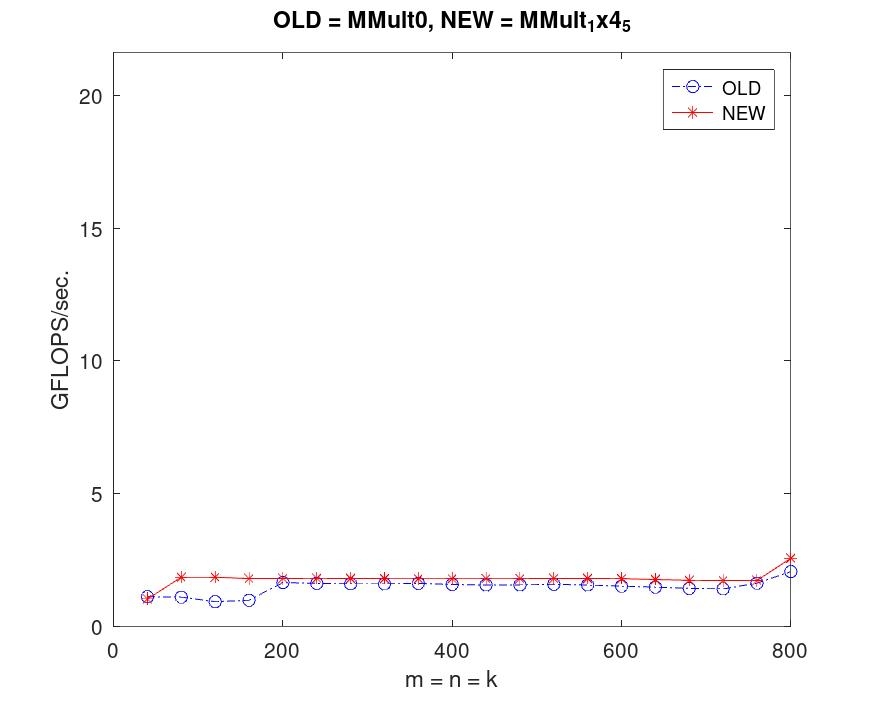
\includegraphics[width=1.0\textwidth]{figure2.jpg}
    \caption{Po optymalizacji 1x4\_5 względem przypadku bazowego}
\end{figure}

\subsection{Optymalizacja 1x4\_6}

\href{https://github.com/flame/how-to-optimize-gemm/blob/master/src/MMult_1x4_6.c}{Kod źródłowy}


\noindent Kolejnym krokiem jest przeniesienie często używanych wartości do rejestrów (np. nowych
wartości dodawanych do macierzy \codeword{C} lub wcześniej wspomnianego \codeword{A(0, p)}).
Skutkuje to znaczącą poprawą.

\begin{figure}[H]
    \centering
    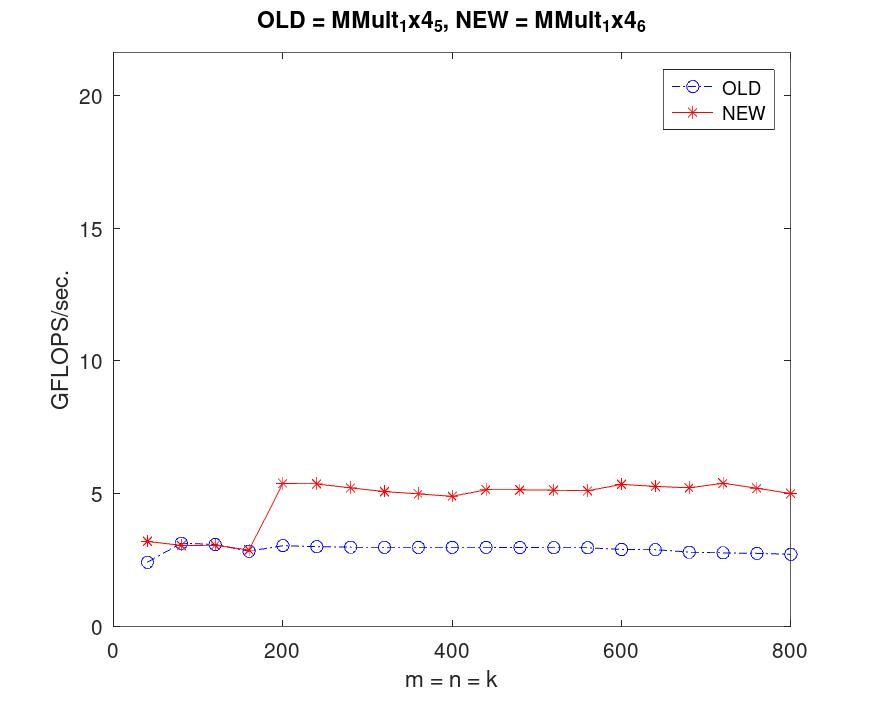
\includegraphics[width=1.0\textwidth]{figure3.jpg}
    \caption{Po optymalizacji 1x4\_6 względem przypadku bazowego}
\end{figure}

\subsection{Optymalizacje 1x4\_7 - 1x4\_9}

\href{https://github.com/flame/how-to-optimize-gemm/blob/master/src/MMult_1x4_9.c}{Kod źródłowy}

Wartości z macierzy \codeword{B} zastąpione zostały wskaźnikami, co zmniejsza narzut indeksowania.
Dodatkowo, rozwinięta została pętla wewnątrz funkcji \codeword{AddDot1x4} oraz użyto \textit{indirect addressing}
na wskaźnikach (zamiast inkrementacji). Poprawa jest marginalna, lub jej nie ma.

\begin{figure}[H]
    \centering
    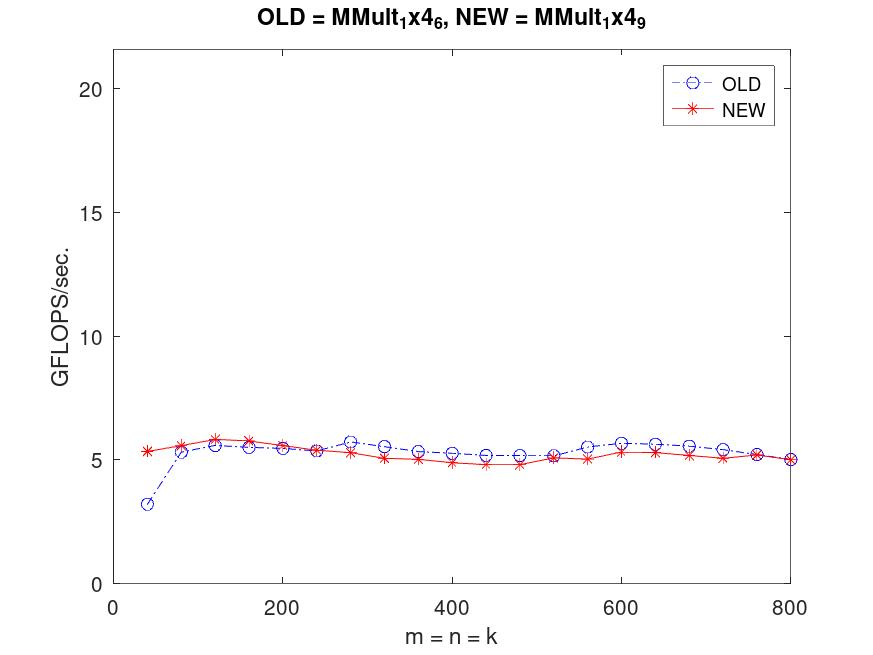
\includegraphics[width=1.0\textwidth]{figure4.jpg}
    \caption{Po optymalizacji 1x4\_9 wzlgędem przypadku bazowego}
\end{figure}

\subsection{Optymalizacje 1 - 4x4\_7}

\href{https://github.com/flame/how-to-optimize-gemm/blob/master/src/MMult_4x4_7.c}{Kod źródłowy}

Tutaj powtórzone zostaną wszystkie poprzednie kroki analogiczne do \textbf{1} - \textbf{1x4\_7},
jednak funkcja \codeword{AddDot1x4} zastąpiona zostanie funkcją \codeword{AddDot4x4} wykonującą
obliczenia dla bloku cztery na cztery elementy macierzy.

\begin{figure}[H]
    \centering
    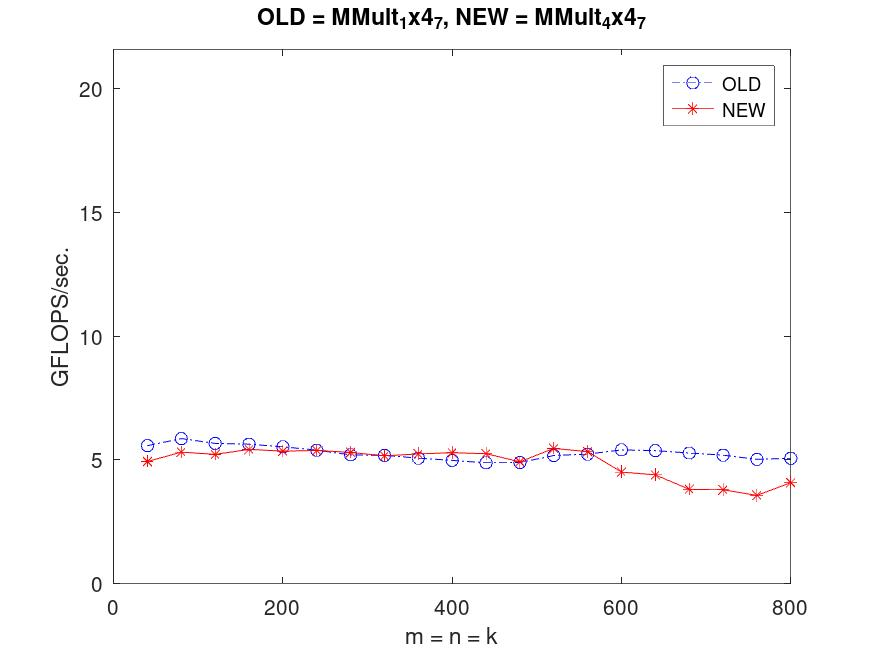
\includegraphics[width=1.0\textwidth]{figure5.jpg}
    \caption{Po optymalizacji 4x4\_7 wzlgędem 1x4\_7}
\end{figure}

\subsection{Optymalizacje 4x4\_8 - 4x4\_9}

\href{https://github.com/flame/how-to-optimize-gemm/blob/master/src/MMult_4x4_9.c}{Kod źródłowy}

Pierwszym krokiem w tej części optymalizacji jest użycie rejestrów do przechowanie elementów
macierzy \codeword{B} w danej iteracji. Kolejny krok to niewielka rearanżacja kolejności
wykonywania obliczeń w przygotowaniu do użycia instrukcji wektorowych. Różnice prawie niezauważalne.

\begin{figure}[H]
    \centering
    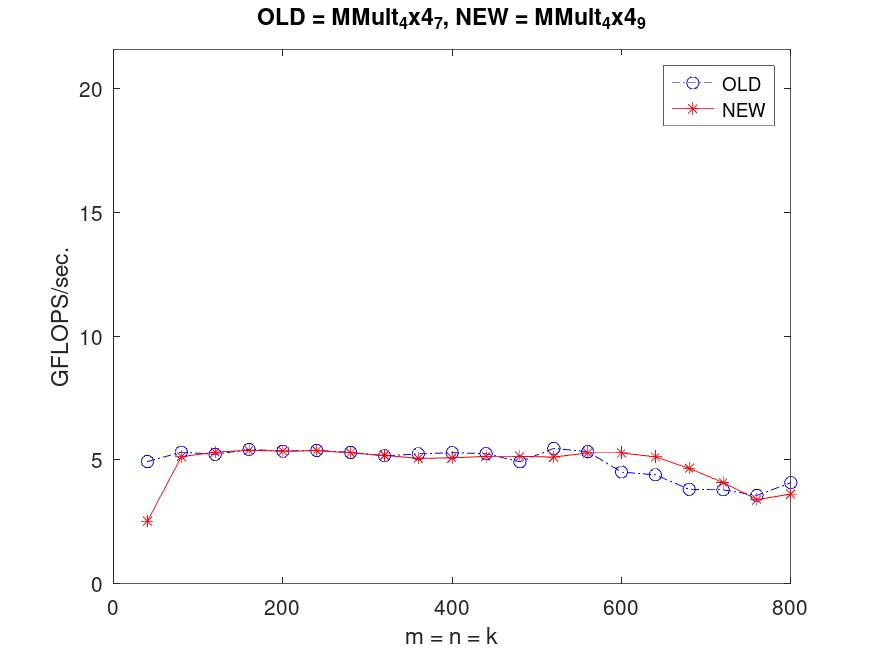
\includegraphics[width=1.0\textwidth]{figure6.jpg}
    \caption{Po optymalizacji 4x4\_9 wzlgędem 4x4\_7}
\end{figure}

\subsection{Optymalizacje 4x4\_10}

\href{https://github.com/flame/how-to-optimize-gemm/blob/master/src/MMult_4x4_10.c}{Kod źródłowy}

Kolejny etap to użycie dedykowanych rejestrów i instrukcji procesora do obliczeń wektorowych (SSE3).
Wartości macierzy zostaną zapisane w 128-bitowych rejestrach (każdy rejestr mieści 2 liczby typu
 \textit{double}), w ośmiu spośród tych rejestórw zostaną zapisane wartości z oblicznego bloku
macierzy \codeword{C}, w czterech aktualnie używane wartości z macierzy \codeword{A} oraz \codeword{B}.
Zastosowanie instrukcji i rejestrów wektorowych przynosi znaczącą poprawę.

\begin{figure}[H]
    \centering
    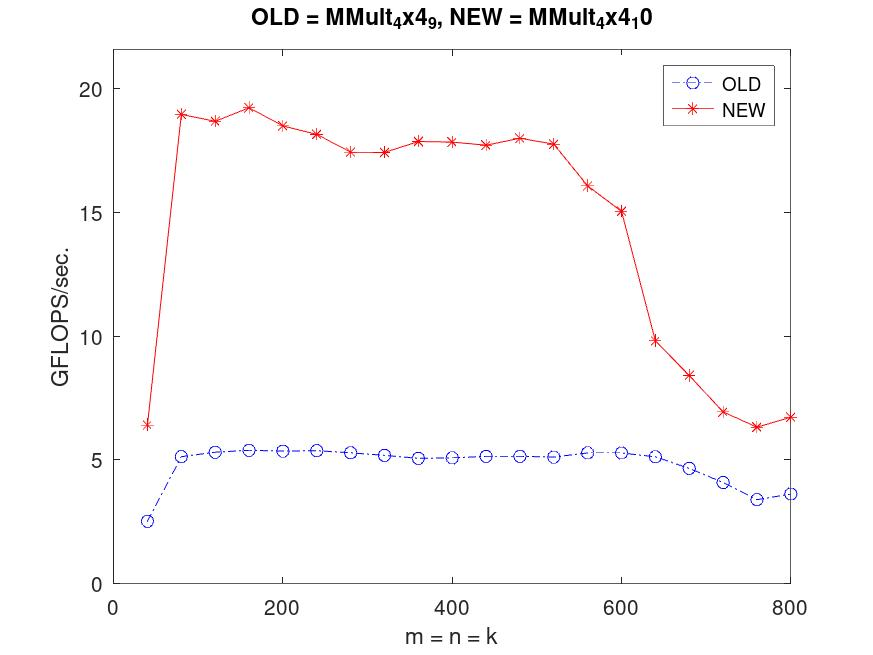
\includegraphics[width=1.0\textwidth]{figure7.jpg}
    \caption{Po optymalizacji 4x4\_10 wzlgędem 4x4\_9}
\end{figure}

\subsection{Optymalizacja 4x4\_11}

\href{https://github.com/flame/how-to-optimize-gemm/blob/master/src/MMult_4x4_11.c}{Kod źródłowy}

Następny krok to wydzielenie głównej rutyny programu, tak żeby operowała na macierzach mieszczących się w \textit{L2 Cache}. Polega to na stworzeniu głównej pętli, która wydziela bloki macierzy \codeword{C}
mieszczące się w \textit{cache}. Następnie, na wydzielonywch blokach wykonuje obliczenia rutyna z poprzednich
optymalizacja operującja na blokach 4x4.Daje to znaczną poprawę dla dużych macierzy, które w całości nie zmieściły by się w \textit{cache}

\begin{figure}[H]
    \centering
    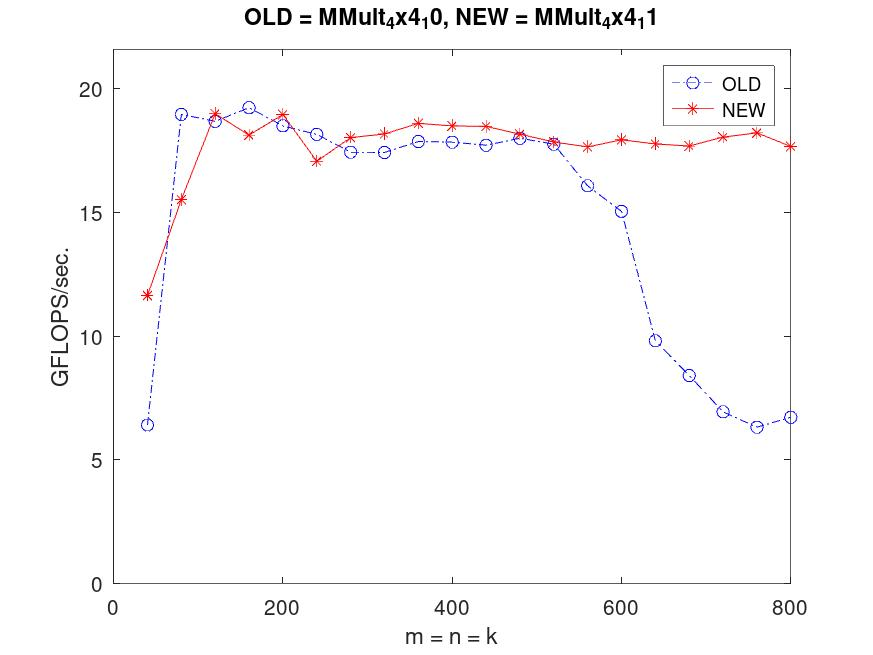
\includegraphics[width=1.0\textwidth]{figure8.jpg}
    \caption{Po optymalizacji 4x4\_11 wzlgędem 4x4\_10}
\end{figure}

\subsection{Optymalizacje 4x4\_12 - 4x4\_15}

\href{https://github.com/flame/how-to-optimize-gemm/blob/master/src/MMult_4x4_15.c}{Kod źródłowy}

Kolejne, końcowe etapy to umieszczenie części macierzy \codeword{A} oraz \codeword{B}, na których
aktualnie wykonywane są obliczenia, w ciągłych blokach pamięci (co pozwoli przychodzić po 
przylegających kawałakch pamięci). Przynosi to niewielką poprawę
(co jest zaskakujące w kontekście tego, jaką poprawę ten krok przyniósł w instrukcji do zadania).

\begin{figure}[H]
    \centering
    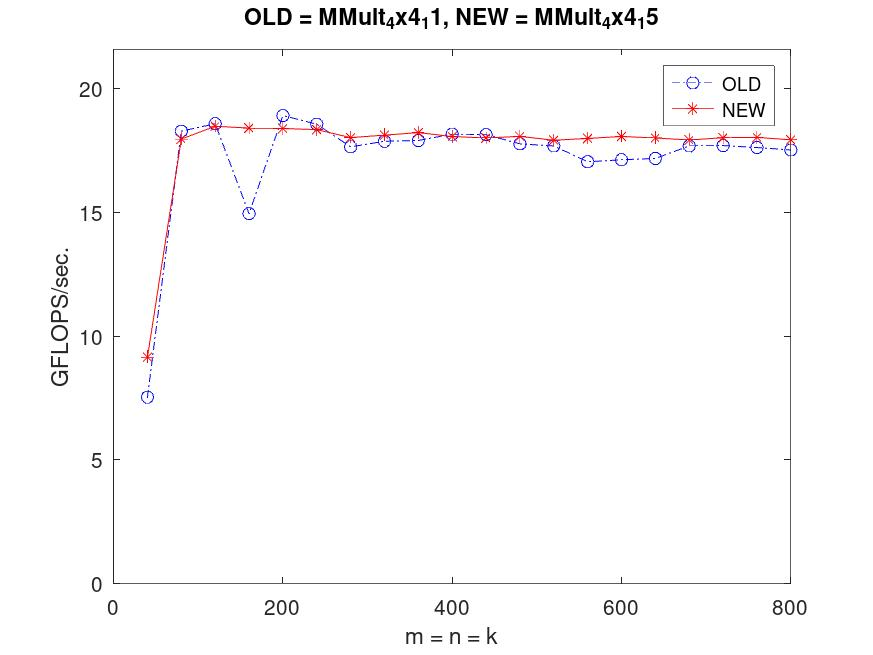
\includegraphics[width=1.0\textwidth]{figure9.jpg}
    \caption{Po optymalizacji 4x4\_15 wzlgędem 4x4\_11}
\end{figure}

\subsection{Optymalizacja AVX}

Ten etap wybiega poza instrukcje zadania. Procesor urządzenia używanego podczas wykonywania zadania
posiada również 256-bitowe rejestry i instrukcje wektorowe AVX, które zostaną użyte do dalszej 
optymalizacji.

\begin{verbatim}
#include <immintrin.h>  // includes AVX, AVX2 intrinsics
...
typedef union
{
  __m256d v;
  double d[4];
} v4df_t;

void AddDot4x4( int k, double *a, int lda,  double *b, int ldb, double *c, int ldc )
{
  int p;
  v4df_t
    c_00_c_30_vreg,    c_01_c_31_vreg,    c_02_c_32_vreg,    c_03_c_33_vreg,
    a_0p_a_3p_vreg,
    b_p0_vreg, b_p1_vreg, b_p2_vreg, b_p3_vreg; 
  __m128d 
    b_temp_vreg;  // to use in _mm256_broadcast_pd

  c_00_c_30_vreg.v = _mm256_setzero_pd();   
  c_01_c_31_vreg.v = _mm256_setzero_pd();
  c_02_c_32_vreg.v = _mm256_setzero_pd(); 
  c_03_c_33_vreg.v = _mm256_setzero_pd(); 

  for ( p=0; p<k; p++ ){
    a_0p_a_3p_vreg.v = _mm256_load_pd( (double *) a );
    a += 4;

    // load the same double value to all of 4 64bit slots in the register
    b_temp_vreg = _mm_loaddup_pd( (double *) b );
    b_p0_vreg.v = _mm256_broadcast_pd(&b_temp_vreg);
    b_temp_vreg = _mm_loaddup_pd( (double *) (b+1) );
    b_p1_vreg.v = _mm256_broadcast_pd(&b_temp_vreg);
    b_temp_vreg = _mm_loaddup_pd( (double *) (b+2) );
    b_p2_vreg.v = _mm256_broadcast_pd(&b_temp_vreg);
    b_temp_vreg = _mm_loaddup_pd( (double *) (b+3) );
    b_p3_vreg.v = _mm256_broadcast_pd(&b_temp_vreg);
    b += 4;

    c_00_c_30_vreg.v = 
      _mm256_add_pd(c_00_c_30_vreg.v, _mm256_mul_pd(a_0p_a_3p_vreg.v, b_p0_vreg.v));
    c_01_c_31_vreg.v = 
      _mm256_add_pd(c_01_c_31_vreg.v, _mm256_mul_pd(a_0p_a_3p_vreg.v, b_p1_vreg.v));
    c_02_c_32_vreg.v = 
      _mm256_add_pd(c_02_c_32_vreg.v, _mm256_mul_pd(a_0p_a_3p_vreg.v, b_p2_vreg.v));
    c_03_c_33_vreg.v = 
      _mm256_add_pd(c_03_c_33_vreg.v, _mm256_mul_pd(a_0p_a_3p_vreg.v, b_p3_vreg.v));
  }

  C( 0, 0 ) += c_00_c_30_vreg.d[0];  C( 0, 1 ) += c_01_c_31_vreg.d[0];  
  C( 0, 2 ) += c_02_c_32_vreg.d[0];  C( 0, 3 ) += c_03_c_33_vreg.d[0]; 

  C( 1, 0 ) += c_00_c_30_vreg.d[1];  C( 1, 1 ) += c_01_c_31_vreg.d[1];  
  C( 1, 2 ) += c_02_c_32_vreg.d[1];  C( 1, 3 ) += c_03_c_33_vreg.d[1]; 

  C( 2, 0 ) += c_00_c_30_vreg.d[2];  C( 2, 1 ) += c_01_c_31_vreg.d[2];  
  C( 2, 2 ) += c_02_c_32_vreg.d[2];  C( 2, 3 ) += c_03_c_33_vreg.d[2]; 

  C( 3, 0 ) += c_00_c_30_vreg.d[3];  C( 3, 1 ) += c_01_c_31_vreg.d[3];  
  C( 3, 2 ) += c_02_c_32_vreg.d[3];  C( 3, 3 ) += c_03_c_33_vreg.d[3]; 
}
\end{verbatim}

Zaskakująco, wydajność działania programu zmniejszyła się, pomimo tego, że w teorii teraz wykonywane
są cztery mnożenia w jednym cyklu zegara, zamiast dwóch. Również warto zauważyć, że przy użyciu
opcji kompilatora \codeword{-march=native} lub \codeword{-mavx2} pozostałe przykłady, np.
MMult\_4x4\_15 zaczęły działać szybciej, co może sugerować, że kompilator wykonuje
dodatkowe optymalizacje z użyciem nowo dostępnych instrukcji procesora. Nie udało się
stwierdzić, co może być powodem pogorszenia wydajności w tym przypadku.

\begin{figure}[H]
    \centering
    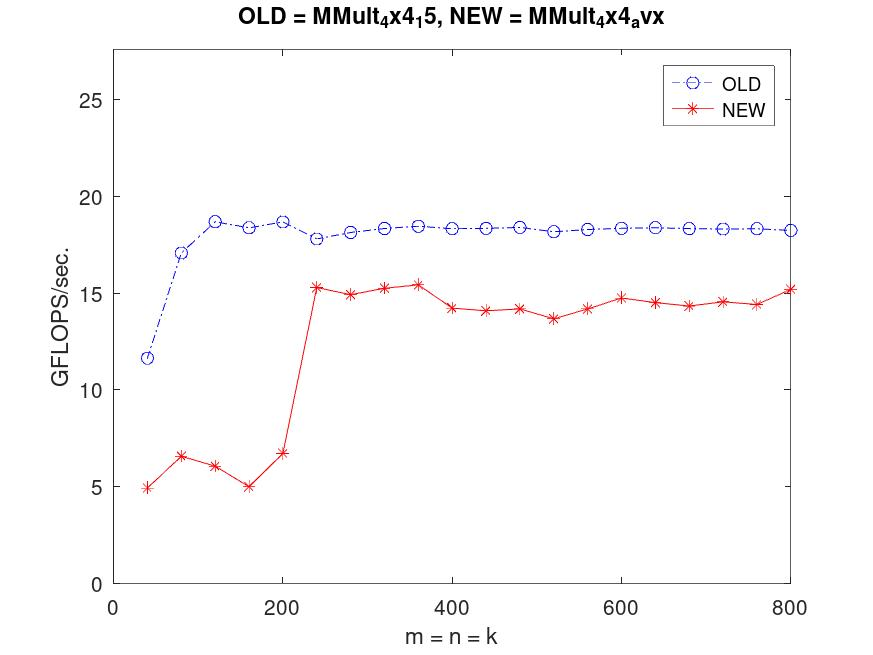
\includegraphics[width=1.0\textwidth]{figure10.jpg}
    \caption{Po optymalizacji 4x4\_avx wzlgędem 4x4\_15}
\end{figure}

\section{Wnioski}

Powyżej przedstawione przykłady pokazują, że relatywnie niewielkim wysiłkiem można znacznie
zoptymalizować działanie dosyć prymitywnego algorytmu. Znajomość i wykorzystanie
niskopoziomowych mechanizmów, takich jak rejestry, cache oraz dedykowane instrukcje
do wykonywania obliczeń wektorowych pozwoliła na znaczne przyspieszenie działania programu.

\begin{figure}[H]
    \centering
    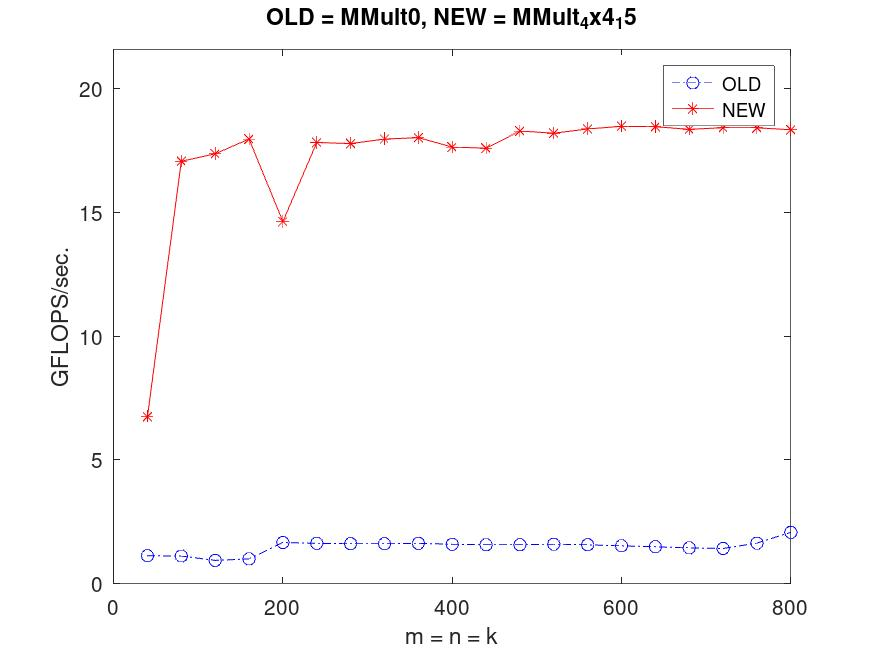
\includegraphics[width=1.0\textwidth]{figure11.jpg}
    \caption{Porównanie wersji bazowej z ostateczną}
\end{figure}

Pokazuje to, jak istotna jest świadomość tego, jakich optymalizacji kompilator dokonuje, jak w rzeczywistości kod jest wykonywany na procesorze, jakie czynniki, potencjalnie niezauważalne, mogą wpłynąć na działanie programu oraz jak można wykorzystywać mechanizmy
specyficzne dla architektury procesora, oraz które spośród tych mechanizmów mogą mieć największy
wpływ na czas działania programu.

\end{document}